\begin{frame}{Kershaw}
  \begin{figure}
  {\setlength{\unitlength}{\textwidth}
  \begin{picture}(1,0.33)
     \put(0.00,0.025){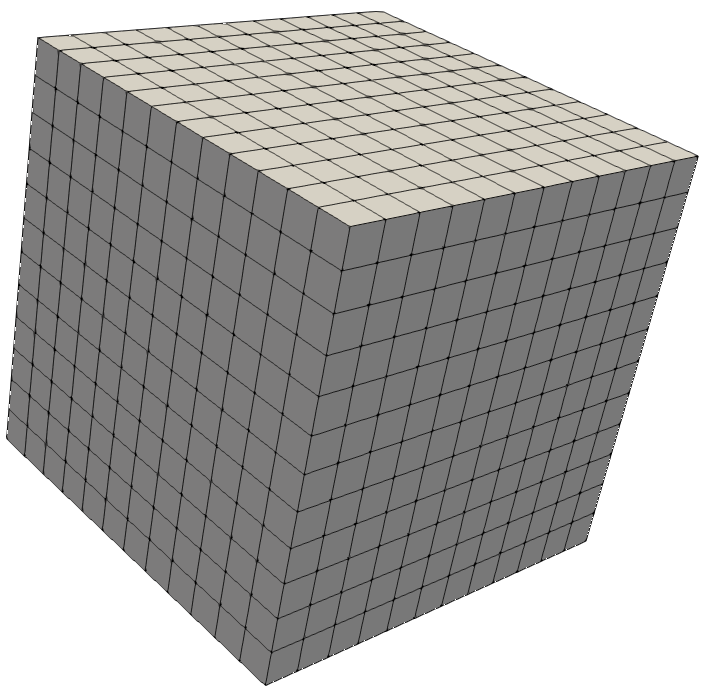
\includegraphics[width=0.33\textwidth]{../figs/kershaw-eps-1.0}}
     \put(0.33,0.025){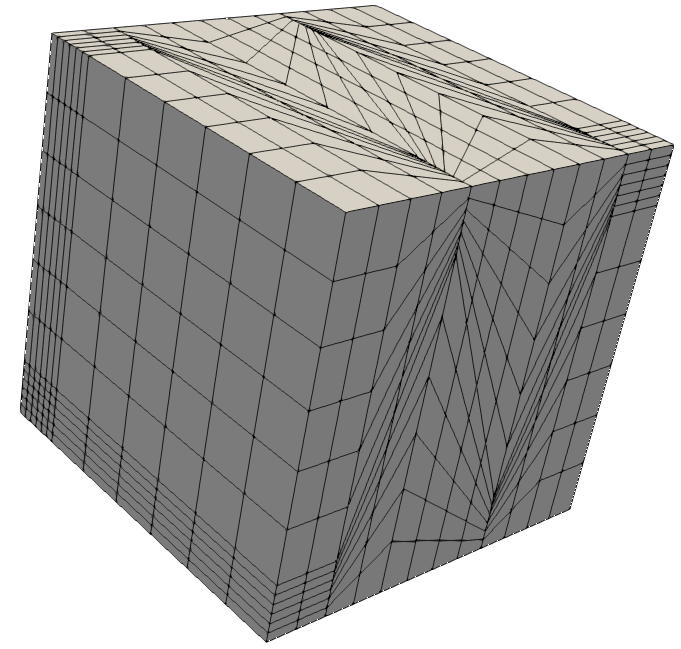
\includegraphics[width=0.33\textwidth]{../figs/kershaw-eps-0.3}}
     \put(0.67,0.025){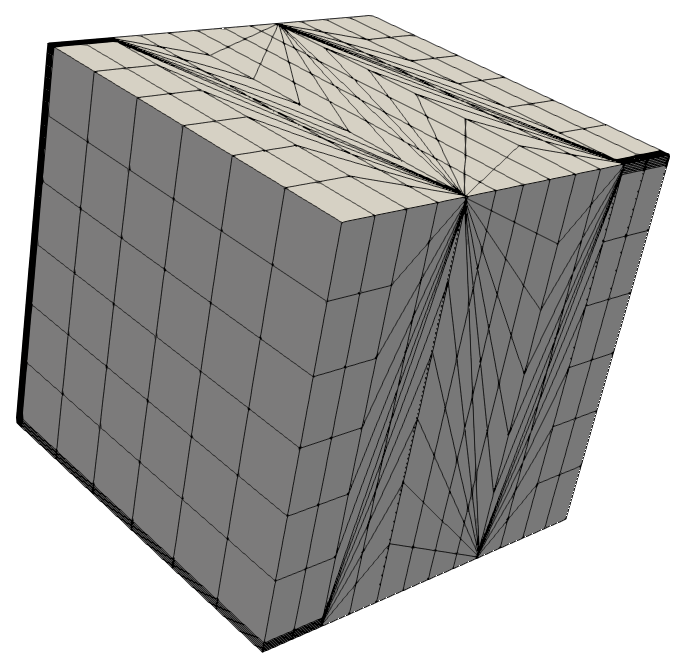
\includegraphics[width=0.33\textwidth]{../figs/kershaw-eps-0.05}}
     \put(0,0.025){\vector(1,0){1}}
     \put(0.4,-0.015){Decreasing $\varepsilon$}
  
     \put(-0.05,0.05){$\varepsilon = 1.0$}
     \put(0.25,0.05){$\varepsilon = 0.3$}
     \put(0.60,0.05){$\varepsilon = 0.05$}
  
  \end{picture}}
  \end{figure}
  Kershaw family of meshes \cite{kolev_ceed_2021,kershaw_differencing_1981} on $\Omega:=[-1/2,1/2]^3$,
  Dirichlet on $\partial\Omega$ with right hand side:
  \begin{equation*}\label{eq:kershaw-rhs}
    f(x,y,z) = 3\pi^2 \sin{(\pi x)}\sin{(\pi y)}\sin{(\pi z)} + g,%(x,y,z),
  \end{equation*}
  where $g(x,y,z)$ is a random, continous vector vanishing on $\partial\Omega$.
  Vary $(E,p)$ for weak scaling and order dependence studies.
  Solution target: $10^{-8}$ relative residual reduction.

\end{frame}
